%%%%%%%%%%%%%%%%%%%%%%%%%%%%%%%%%%%%%%%%%
% baposter Portrait Poster
% LaTeX Template
% Version 1.0 (15/5/13)
%
% Created by:
% Brian Amberg (baposter@brian-amberg.de)
%
% This template has been downloaded from:
% http://www.LaTeXTemplates.com
%
% License:
% CC BY-NC-SA 3.0 (http://creativecommons.org/licenses/by-nc-sa/3.0/)
%
%%%%%%%%%%%%%%%%%%%%%%%%%%%%%%%%%%%%%%%%%

%----------------------------------------------------------------------------------------
%	PACKAGES AND OTHER DOCUMENT CONFIGURATIONS
%----------------------------------------------------------------------------------------

\documentclass[a0paper,portrait]{baposter}

\usepackage[font=small,labelfont=bf]{caption} % Required for specifying captions to tables and figures
\usepackage{booktabs} % Horizontal rules in tables
\usepackage{relsize} % Used for making text smaller in some places
%\usepackage{inputenc}
\graphicspath{{figures/}} % Directory in which figures are stored

\definecolor{bordercol}{RGB}{40,40,40} % Border color of content boxes
\definecolor{headercol1}{RGB}{186,215,230} % Background color for the header in the content boxes (left side)
\definecolor{headercol2}{RGB}{80,80,80} % Background color for the header in the content boxes (right side)
\definecolor{headerfontcol}{RGB}{0,0,0} % Text color for the header text in the content boxes
\definecolor{boxcolor}{RGB}{186,215,230} % Background color for the content in the content boxes

\begin{document}

\background{ % Set the background to an image (background.pdf)
\begin{tikzpicture}[remember picture,overlay]
\draw (current page.north west)+(-3em,3em) node[anchor=north west]
{
\includegraphics[height=1.1\textheight]{background}};
\end{tikzpicture}
}

\begin{poster}{
grid=false,
borderColor=bordercol, % Border color of content boxes
headerColorOne=headercol1, % Background color for the header in the content boxes (left side)
headerColorTwo=headercol2, % Background color for the header in the content boxes (right side)
headerFontColor=headerfontcol, % Text color for the header text in the content boxes
boxColorOne=boxcolor, % Background color for the content in the content boxes
headershape=rounded, % Specify the rounded corner in the content box headers
headerfont=\Large\sf\bf, % Font modifiers for the text in the content box headers
textborder=rectangle,
background=user,
headerborder=open, % Change to closed for a line under the content box headers
boxshade=plain
}
{}
%
%----------------------------------------------------------------------------------------
%	TITLE AND AUTHOR NAME
%----------------------------------------------------------------------------------------
%
{\sf\bf \Huge Dynamic identification of brain networks by Bayesian tracking of electrophysiological data } % Poster title
{\vspace{1em} Author names and order to be decided\\ % Author names
{\smaller corresponding author's email id}} % Author email addresses
{
\includegraphics[scale=0.08]{figures/logo}} % University/lab logo

%----------------------------------------------------------------------------------------
%	INTRODUCTION
%----------------------------------------------------------------------------------------

\headerbox{Introduction}{name=introduction,column=0,row=0}{
\begin{enumerate}
\item \textbf{Decoding functional brain networks} is key to understanding not only \textbf{higher order cognitive functions}, but also in pathologies like \textbf{epilepsy}.
\item \textbf{Electroencephalography} (EEG) and \textbf{magnetoencephalography} (MEG) measure electric and magnetic fields due to the electrical activity of neurons in the brain.
\item Both EEG and MEG are \textbf{non-invasive methods} and have \textbf{sub-millisecond temporal resolution}.
\item However, \textbf{neither of the recording modalities} give any \textbf{information} about the underlying \textbf{network structure}.
\item In our project \textbf{BrainTrack}, we propose a novel method to estimate functional brain connectivity using \textbf{Bayesian tracking}.
\end{enumerate}


}

%----------------------------------------------------------------------------------------
%	SIGNIFICANCE OF RESEARCH
%----------------------------------------------------------------------------------------

\headerbox{Significance of research}{name=significance,column=0,below=introduction}{
\begin{enumerate}
\item Pathologies like epilepsy can be considered as \textbf{network disorders}.
\item Tools for the characterization of epileptic activity as a \textbf{dynamic functional network} can greatly aid the accurate \textbf{localization} of \textbf{epileptic foci}.
\item Many higher order cognitive functions rely of \textbf{dynamic reconfiguration} of \textbf{functional brain networks}.
\item Thus, dynamic functional connectivity estimation can be of great importance to \textbf{cognitive and systems-level neuroscience}.
\item Also, our method allows for real-time connectivity estimation, which can greatly benefit \textbf{neurofeedback} experiments.
\end{enumerate}

}

%----------------------------------------------------------------------------------------
%	RESEARCH OBJECTIVES
%----------------------------------------------------------------------------------------

\headerbox{Research objectives}{name=obj,column=0,span=1,below=significance}{
\begin{enumerate}
\item To develop a common \textbf{statistical framework} for the source and connectivity estimation.
\item To incorporate of \textbf{soft priors} such as connectivity information from diffusion tensor imaging data.
\item To offer \textbf{real-time} estimation of brain connectivity for neurofeedback experiments.
\end{enumerate}

}



%----------------------------------------------------------------------------------------
%	RESSEARCH METHODOLOGY
%----------------------------------------------------------------------------------------
\headerbox{Research methodology}{name=method,column=1,span=2}{
\begin{description}

\item \textbf{Forward modeling}

\begin{enumerate}
\item Individual magnetic resonance images (MRI) will be segmented using \textbf{FreeSurfer} software.
\item Realistic head model including white matter, grey matter, cerebrospinal fluid, skull and scalp will be constructed using boundary element method (BEM).
\item Lead field matrix mapping the sources to EEG/MEG sensors will be derived using the MEG/EEG analysis software \textbf{MNE}.
\end{enumerate}

\item \textbf{Preprocessing of EEG/MEG data}
\begin{enumerate}
\item EEG/MEG will be preprocessed using the \textbf{FieldTrip} toolbox.
\item Independent component analysis will be used to remove ocular artifacts.
\item Signal space separation will be used to enhance the quality of MEG data.
\end{enumerate}

\item \textbf{Inversion and connectivity estimation}
\begin{enumerate}
\item Spatio-temporal particle filter algorithm will be developed and implemented  to estimate network structure along with neural source parameters.
\item Rao-Blackwellization will be used to ensure efficiency with high state dimensions.
\item The estimation of source signals $X_t$ and connectivity parameters $\theta_t$ from the observations $Y_{1:t}$ will be given by the posterior probability distribution $p(X_t, \theta_t | Y_{1:t})$.
\end{enumerate}

\end{description}
}

%----------------------------------------------------------------------------------------
%	RESSEARCH FRAMEWORK
%----------------------------------------------------------------------------------------

\headerbox{Research framework}{name=framework,span=2,column=1,row=0,below=method}{ % To reduce this block to 1 column width, remove 'span=2'
\begin{center}
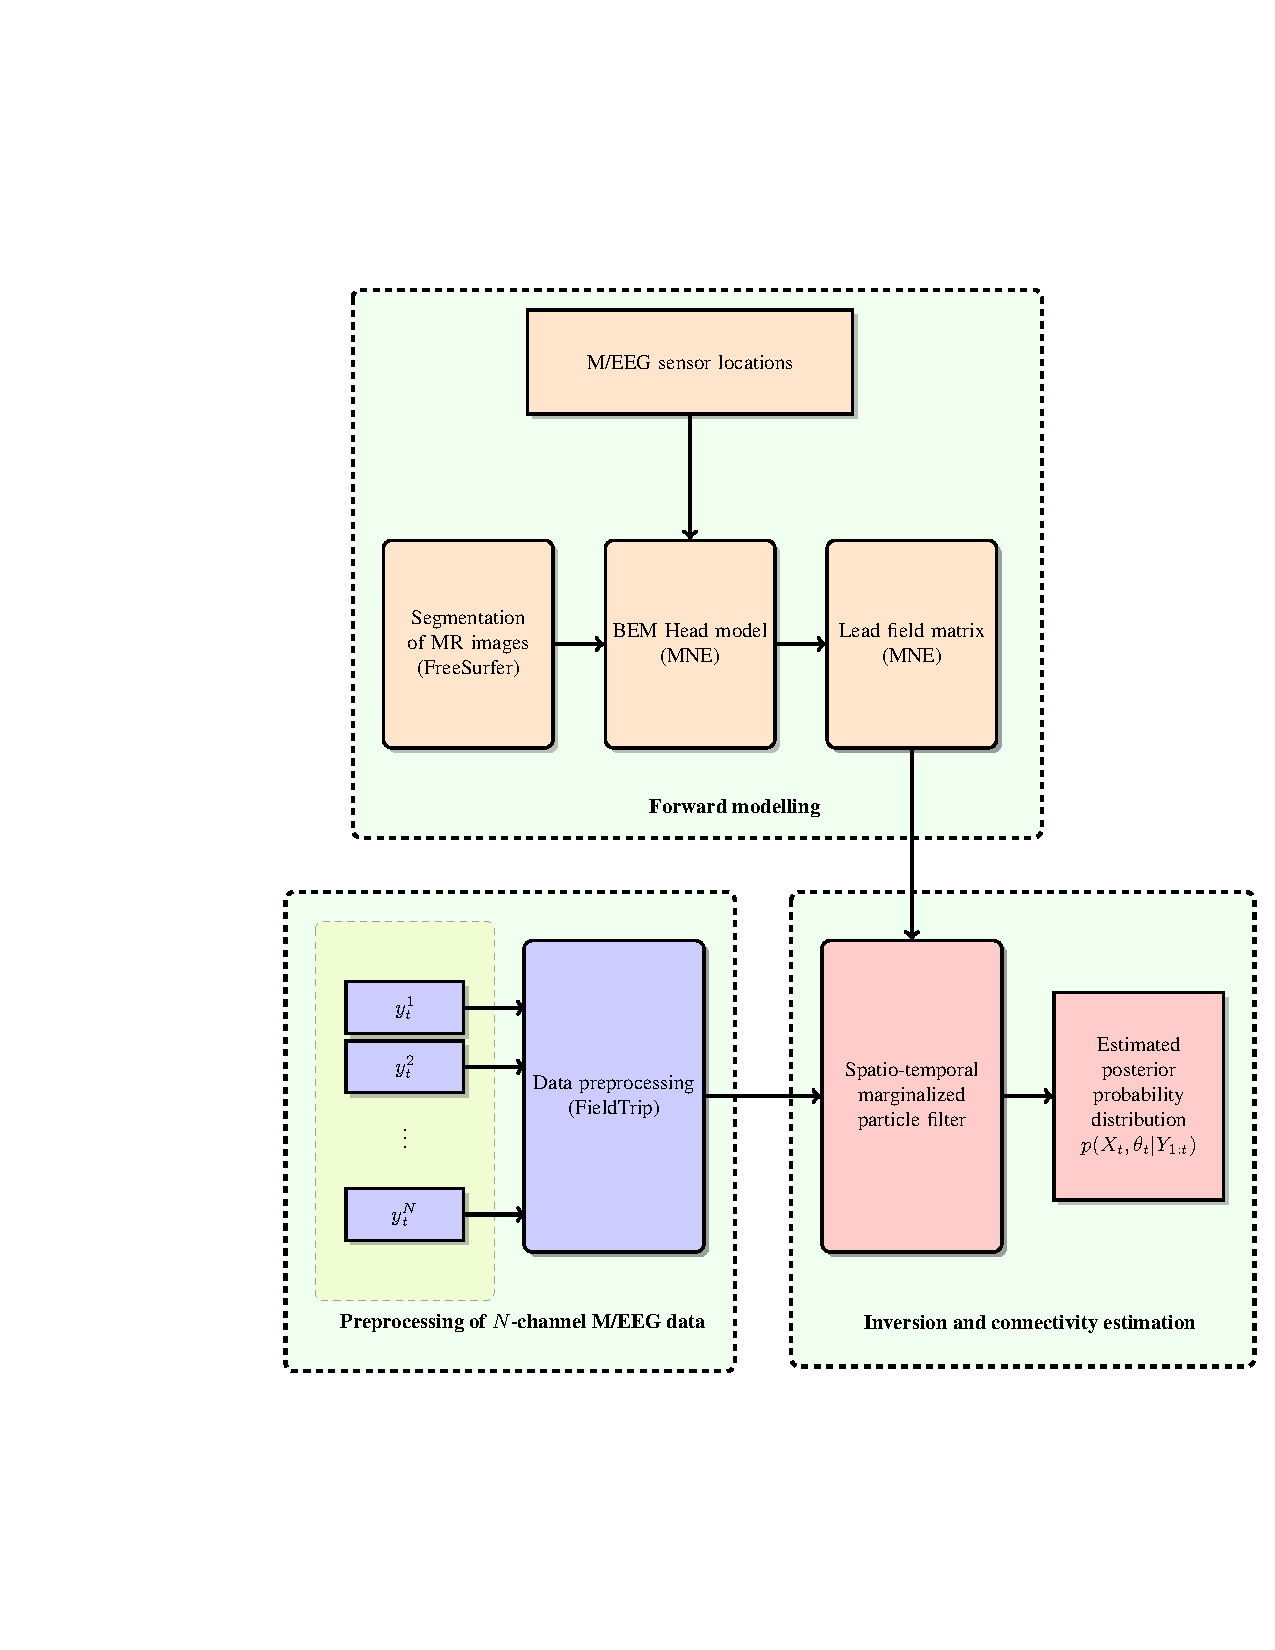
\includegraphics[scale=0.42,resolution=720]{framework.pdf}
\captionof{figure}{Research framework representing the workflow of different modules}
\label{fig1}
\end{center}
}



%----------------------------------------------------------------------------------------
%	EXPECTED RESULTS AND IMPACT
%----------------------------------------------------------------------------------------

\headerbox{Expected results and impact}{name=results2,span=3,column=0,below=obj}{ % To reduce this block to 1 column width, remove 'span=2'
\begin{enumerate}
\item An on-line platform for \textbf{accurate and real-time} estimation of functional brain connectivity from electrophysiological data. 
\item \textbf{Better characterization} of spreading of pathological activity in \textbf{network disorders} like epilepsy.
\item \textbf{Neurofeedback} based on functional brain networks.
\item The results of BrainTrack project will find quick acceptance within the EEG/MEG community, among \textbf{cognitive neuroscientists} and as well as \textbf{clinical researchers}.
\end{enumerate}
}

%----------------------------------------------------------------------------------------

\end{poster}

\end{document}